%%%%%%%%%%%%%%%%%%%%%%%%%%%%%%%%%%%%%%%%%
% Beamer Presentation
% LaTeX Template
% Version 1.0 (10/11/12)
%
% This template has been downloaded from:
% http://www.LaTeXTemplates.com
%
% License:
% CC BY-NC-SA 3.0 (http://creativecommons.org/licenses/by-nc-sa/3.0/)
%
%%%%%%%%%%%%%%%%%%%%%%%%%%%%%%%%%%%%%%%%%

%----------------------------------------------------------------------------------------
%	PACKAGES AND THEMES
%----------------------------------------------------------------------------------------

\documentclass[aspectratio=169]{beamer}

\mode<presentation> {

\usetheme{CambridgeUS}

}

\usepackage{color}
\usepackage{graphicx} % Allows including images
\usepackage{url}
\usepackage{hyperref}
\usepackage{algorithm2e}
\usepackage{tikz}

\usetikzlibrary{automata,positioning,arrows,chains,fit,shapes}

\DontPrintSemicolon

\DeclareGraphicsExtensions{.png}

\setlength{\parskip}{1em}

%----------------------------------------------------------------------------------------
%	TITLE PAGE
%----------------------------------------------------------------------------------------

\title[Complexity theory]{Topics in Quantum Engineering Presentation:\\Complexity Theory} % The short title appears at the bottom of every slide, the full title is only on the title page

\author{Dominic Moylett} % Your name
\institute[University of Bristol] % Your institution as it will appear on the bottom of every slide, may be shorthand to save space
{
University of Bristol \\ % Your institution for the title page
\medskip
\textit{dominic.moylett@bristol.ac.uk} % Your email address
}
\date{\today} % Date, can be changed to a custom date

\begin{document}

\begin{frame}
\titlepage % Print the title page as the first slide
\end{frame}

%----------------------------------------------------------------------------------------
%	PRESENTATION SLIDES
%----------------------------------------------------------------------------------------

%------------------------------------------------
\section{Introduction: What is complexity theory?}
%------------------------------------------------

\begin{frame}
\frametitle{Complexity theory in a nutshell}
\centerline{``How hard can it be?'', {\em Clarkson, Hammond and May}}
\end{frame}

\begin{frame}
\frametitle{What is complexity theory?}
Complexity theory is the study of how difficult it is to solve a problem with a computer.
\end{frame}

\begin{frame}
\frametitle{What is complexity theory?}
Complexity theory is the study of how {\color{red} difficult} it is to solve a problem with a computer.

How do we measure difficulty?
\end{frame}

\begin{frame}
\frametitle{What is complexity theory?}
Complexity theory is the study of how difficult it is to solve a {\color{red} problem} with a computer.

What is a problem?
\end{frame}

\begin{frame}
\frametitle{What is complexity theory?}
Complexity theory is the study of how difficult it is to solve a problem with a {\color{red} computer}.

What is a computer?
\end{frame}

\begin{frame}
\frametitle{Structure of part one}
\begin{itemize}
    \item What is a computer?
    \item What is a problem?
    \item How do we measure difficulty?
\end{itemize}
\end{frame}

%------------------------------------------------
\section{What is a computer?}
%------------------------------------------------

\begin{frame}
\frametitle{Our model of a computer}
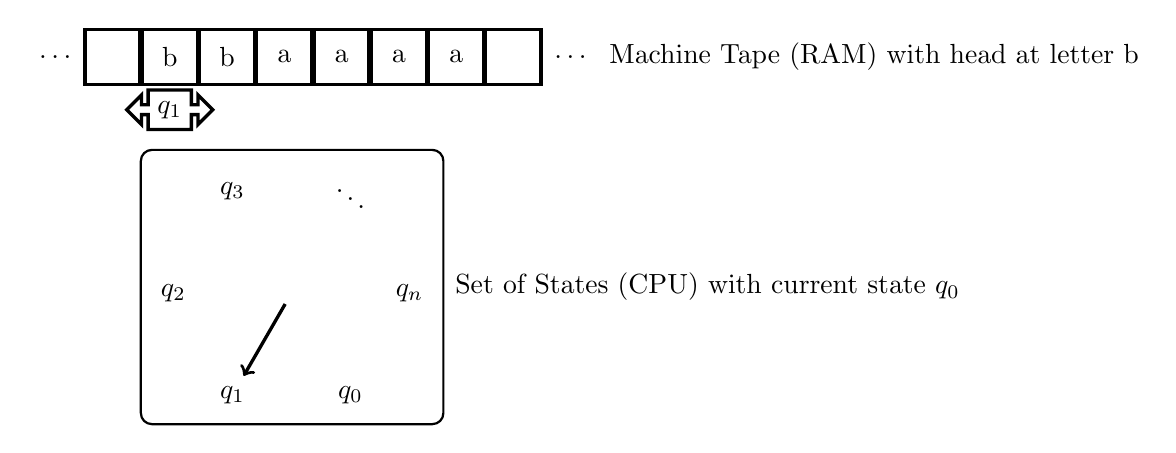
\begin{tikzpicture}
\tikzstyle{every path}=[very thick]

\edef\sizetape{0.7cm}
\tikzstyle{tmtape}=[draw,minimum size=\sizetape]
\tikzstyle{tmhead}=[arrow box,draw,minimum size=.5cm,arrow box
arrows={east:.25cm, west:0.25cm}]

%% Draw TM tape
\begin{scope}[start chain=1 going right,node distance=-0.15mm]
    \node [on chain=1,tmtape,draw=none] {$\ldots$};
    \node [on chain=1,tmtape] {};
    \node [on chain=1,tmtape] (input) {b};
    \node [on chain=1,tmtape] {b};
    \node [on chain=1,tmtape] {a};
    \node [on chain=1,tmtape] {a};
    \node [on chain=1,tmtape] {a};
    \node [on chain=1,tmtape] {a};
    \node [on chain=1,tmtape] {};
    \node [on chain=1,tmtape,draw=none] {$\ldots$};
    \node [on chain=1] {Machine Tape (RAM) with head at letter b};
\end{scope}

%% Draw TM Finite Control
\begin{scope}
[shift={(3cm,-3cm)},start chain=circle placed {at=(-\tikzchaincount*60:1.5)}]
\foreach \i in {q_0,q_1,q_2,q_3,\ddots,q_n}
	\node [on chain] {$\i$};

% Arrow to current state
\node (center) {};
\draw[->] (center) -- (circle-2);

\node[rounded corners,draw=black,thick,fit=(circle-1) (circle-2) (circle-3) 
      (circle-4) (circle-5) (circle-6),
			label=right:Set of States (CPU) with current state $q_0$] (fsbox)
		{};
\end{scope}

%% Draw TM head below (input) tape cell
\node [tmhead,yshift=-.3cm] at (input.south) (head) {$q_1$};

\end{tikzpicture}\footnote{\url{http://www.texample.net/tikz/examples/turing-machine-2/}}
\end{frame}

\begin{frame}
\frametitle{Formal definition of a computer}
A Turing Machine $(TM)$ is specified as a tuple of seven components $(Q, \Sigma, \Gamma, q_0, q_{accept}, q_{reject})$:

\begin{itemize}
	\item $Q$ is the set of all possible states
	\item $\Sigma$ is the input alphabet for the tape. Note that $\Sigma$ cannot contain the blank symbol $\sqcup$
	\item $\Gamma$ is tape alphabet, where $\Sigma \subseteq \Gamma$ and $\sqcup \in \Gamma$
	\item $q_0 \in Q$ is the start state
	\item $q_{accept} \in Q$ is the accept state
	\item $q_{reject} \in Q$ is the reject state, where $q_{reject} \neq q_{accept}$
	\item $\delta: Q \times \Gamma \to Q \times \Sigma \times \{L, R\}$ is the transition function
\end{itemize}
\end{frame}

\begin{frame}
\frametitle{But how do we run it?}
The majority of computation time is spent repeating the following loop. Note that $T_h$ is the $h$-th cell of the tape.
\begin{algorithm}[H]
$q = q_0$\\
$h = 0$\\
$T = w$ \tcp*{Tape starts as just input, followed by blank cells}
\While{$q \notin \{q_{accept}, q_{reject}\}$}{
	$(q, h, i) = \delta(q, T_h)$\\
	\eIf{$i = L$}{$h = h - 1$ \tcp*{Move tape head to the left}}
	{$h = h + 1$ \tcp*{Move tape head to the right}}
}
\end{algorithm}
\end{frame}

\begin{frame}
\frametitle{What happens when it stops?}
When we reach either the {\em accept} or {\em reject} state, the machine has {\em halted}.

If the machine {\em accepted}, then the machine accepts and the contents of the tape, denoted $M(w)$, is returned.

If the machine {\em rejected}, then the machine rejects and nothing is returned.
\end{frame}

\begin{frame}
\frametitle{What can we store in a machine's memory?}
\begin{itemize}
	\item<1-> Integers
	\item<2-> Rational numbers
	\item<3-> Floating point numbers
	\item<4-> Boolean (True/False) statements
	\item<5-> Text
	\item<6-> Graphs
	\item<7-> Other machines
\end{itemize}
\end{frame}

\begin{frame}
\frametitle{Universal Turing Machines}
Turing showed in his PhD thesis that we could represent any $TM$ after any number of transitions -- including current state, tape contents and position of tape head -- as an integer.

Not only that, but we could manipulate this integer such that it matched performing the next step of the computation.

This gave way to Universal Turing Machines; machines capable of running any $TM$ given to them.
\end{frame}

\begin{frame}
\frametitle{The Church-Turing Thesis}
\centerline{``[A]ll effectively calculable sequences are computable'', {\em Turing}}
\end{frame}

\begin{frame}
\frametitle{Quiz Time!}

\begin{center}
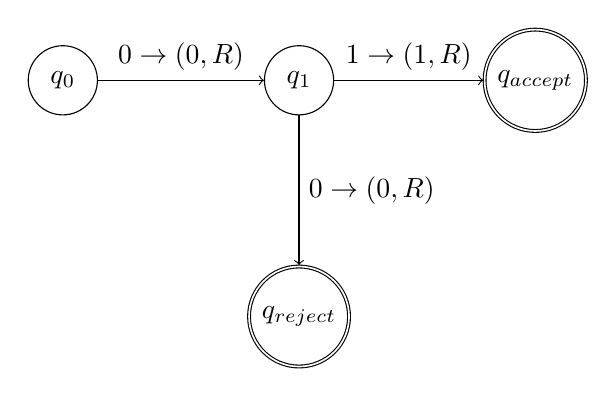
\begin{tikzpicture}[node distance=3cm,on grid,auto]
    \node[state] (q0) at (0,0) {$q_0$};
    \node[state] (q1) [right of=q0] {$q_1$};
    \node[accepting,state] (qaccept) [right of=q1] {$q_{accept}$};
    \node[accepting,state] (qreject) [below of=q1] {$q_{reject}$};
    \path[->]
        (q0) edge node {$0 \to (0, R)$} (q1)
        (q1) edge node {$1 \to (1, R)$} (qaccept)
        (q1) edge node {$0 \to (0, R)$} (qreject);
\end{tikzpicture}
\end{center}

Question: Does $M(01)$ accept or reject?
\end{frame}

\begin{frame}[noframenumbering]
\frametitle{Quiz Time!}

\begin{center}
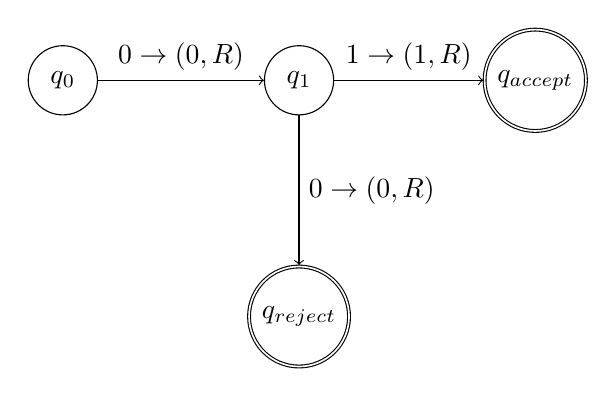
\begin{tikzpicture}[node distance=3cm,on grid,auto]
    \node[state] (q0) at (0,0) {$q_0$};
    \node[state] (q1) [right of=q0] {$q_1$};
    \node[accepting,state] (qaccept) [right of=q1] {$q_{accept}$};
    \node[accepting,state] (qreject) [below of=q1] {$q_{reject}$};
    \path[->]
        (q0) edge node {$0 \to (0, R)$} (q1)
        (q1) edge node {$1 \to (1, R)$} (qaccept)
        (q1) edge node {$0 \to (0, R)$} (qreject);
\end{tikzpicture}
\end{center}

Answer: $M(01)$ accepts!
\end{frame}

\begin{frame}
\frametitle{Quiz Time!}

\begin{center}
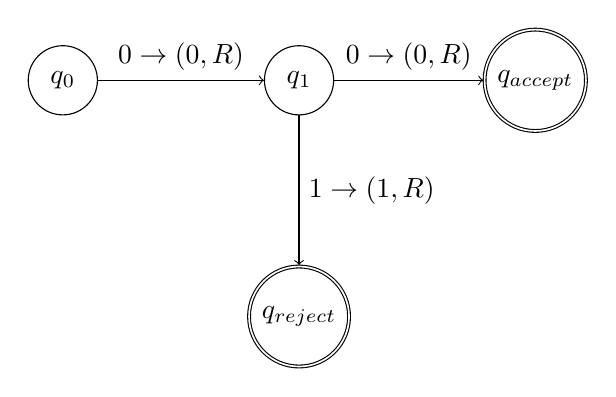
\begin{tikzpicture}[node distance=3cm,on grid,auto]
    \node[state] (q0) at (0,0) {$q_0$};
    \node[state] (q1) [right of=q0] {$q_1$};
    \node[accepting,state] (qaccept) [right of=q1] {$q_{accept}$};
    \node[accepting,state] (qreject) [below of=q1] {$q_{reject}$};
    \path[->]
        (q0) edge node {$0 \to (0, R)$} (q1)
        (q1) edge node {$0 \to (0, R)$} (qaccept)
        (q1) edge node {$1 \to (1, R)$} (qreject);
\end{tikzpicture}
\end{center}

Question: Does $M(01)$ accept or reject?
\end{frame}

\begin{frame}[noframenumbering]
\frametitle{Quiz Time!}

\begin{center}
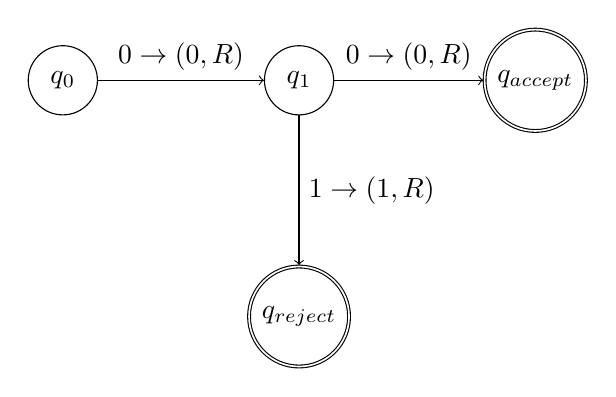
\begin{tikzpicture}[node distance=3cm,on grid,auto]
    \node[state] (q0) at (0,0) {$q_0$};
    \node[state] (q1) [right of=q0] {$q_1$};
    \node[accepting,state] (qaccept) [right of=q1] {$q_{accept}$};
    \node[accepting,state] (qreject) [below of=q1] {$q_{reject}$};
    \path[->]
        (q0) edge node {$0 \to (0, R)$} (q1)
        (q1) edge node {$0 \to (0, R)$} (qaccept)
        (q1) edge node {$1 \to (1, R)$} (qreject);
\end{tikzpicture}
\end{center}

Answer: $M(01)$ rejects!
\end{frame}

\begin{frame}
\frametitle{Quiz Time!}

\begin{center}
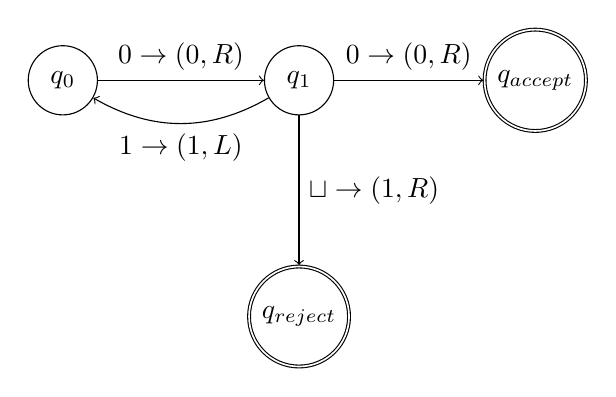
\begin{tikzpicture}[node distance=3cm,on grid,auto]
    \node[state] (q0) at (0,0) {$q_0$};
    \node[state] (q1) [right of=q0] {$q_1$};
    \node[accepting,state] (qaccept) [right of=q1] {$q_{accept}$};
    \node[accepting,state] (qreject) [below of=q1] {$q_{reject}$};
    \path[->]
        (q0) edge node {$0 \to (0, R)$} (q1)
        (q1) edge node {$0 \to (0, R)$} (qaccept)
        (q1) edge node {$\sqcup \to (1, R)$} (qreject)
        (q1) edge [bend left] node {$1 \to (1, L)$} (q0);
\end{tikzpicture}
\end{center}

Question: Does $M(01)$ accept or reject?
\end{frame}

\begin{frame}[noframenumbering]
\frametitle{Quiz Time!}

\begin{center}
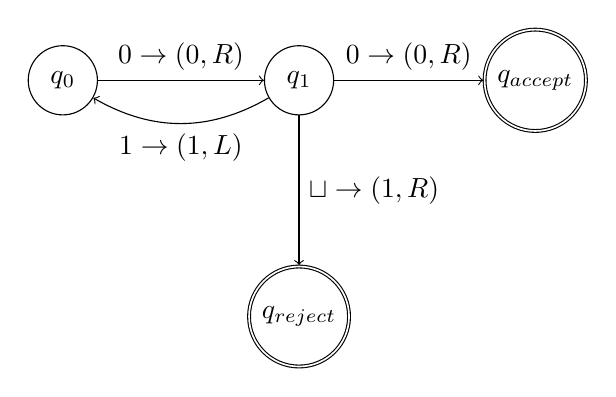
\begin{tikzpicture}[node distance=3cm,on grid,auto]
    \node[state] (q0) at (0,0) {$q_0$};
    \node[state] (q1) [right of=q0] {$q_1$};
    \node[accepting,state] (qaccept) [right of=q1] {$q_{accept}$};
    \node[accepting,state] (qreject) [below of=q1] {$q_{reject}$};
    \path[->]
        (q0) edge node {$0 \to (0, R)$} (q1)
        (q1) edge node {$0 \to (0, R)$} (qaccept)
        (q1) edge node {$\sqcup \to (1, R)$} (qreject)
        (q1) edge [bend left] node {$1 \to (1, L)$} (q0);
\end{tikzpicture}
\end{center}

Answer: $M(w)$ doesn't halt.
\end{frame}

\begin{frame}
\frametitle{The halting problem}
You might think it would be useful if we could tell when a machine was going to halt.

Formally, we want a $TM\, H$ such that given $M \in TM \text{ and } w \in \Sigma_M^*$:

\begin{itemize}
	\item $H(M, w)$ halts in the accept state if $M(w)$ halts and
	\item $H(M, w)$ halts in the reject state if $M(w)$ does not halt.
\end{itemize}

Sadly, Turing proved that such a machine is impossible.

There are many other unsolvable problems as well, within the area of {\bf computability theory}. We will not cover this area, but some reading on the subject is suggested at the end.
\end{frame}

\begin{frame}
\frametitle{Nondeterminism: Spot the difference!}
A Nondeterministic Turing Machine $(NTM)$ is specified as a tuple of seven components $(Q, \Sigma, \Gamma, q_0, q_{accept}, q_{reject})$:

\begin{itemize}
	\item $Q$ is the set of all possible states
	\item $\Sigma$ is the input alphabet for the tape. Note that $\Sigma$ cannot contain the blank symbol $\sqcup$
	\item $\Gamma$ is tape alphabet, where $\Sigma \subseteq \Gamma$ and $\sqcup \in \Gamma$
	\item $q_0 \in Q$ is the start state
	\item $q_{accept} \in Q$ is the accept state
	\item $q_{reject} \in Q$ is the reject state, where $q_{reject} \neq q_{accept}$
	\item $\delta: Q \times \Gamma \to (Q \times \Sigma \times \{L, R\})^*$ is the transition function
\end{itemize}
\end{frame}

\begin{frame}
\frametitle{What, what's the difference?}
$NTM$s are different because of the transition function.

In deterministic $TMs$, the transition goes from one machine setup to another.

In $NTM$s, the transition function goes from one to many setups.

These setups are run simultaneously, and the machine accepts if one setup halts in an accepting state, or rejects if all setups halt in the rejecting state.
\end{frame}

\begin{frame}
\frametitle{Computation Tree}

\end{frame}

\begin{frame}
\frametitle{Power of Nondeterminism}
Note that a $TM$s only transition from one machine setup to another, while $NTM$s transition from one to many.

From this, we can conclude that any $TM$ is by definition also an $NTM$.

Question: Is there any problem that can be solved by an $NTM$ that cannot be solved by a $TM$?
\end{frame}

\begin{frame}
\frametitle{Using $TM$s to simulate $NTM$s}
Recall the computation tree:

We can use Breadth-First Search to search every branch until we find one that halts in an accept state.
\end{frame}

\begin{frame}
\frametitle{Structure of part one}
\begin{itemize}
    \item What is a computer? {\em Deterministic Turing Machine, Nondeterministic Turing Machine}
    \item What is a problem?
    \item How do we measure difficulty?
\end{itemize}
\end{frame}

%------------------------------------------------
\section{What is a problem?}
%------------------------------------------------

\begin{frame}
\frametitle{Describing problems as languages}
A {\em language} $L$ is a (potentially infinite) set.

Example languages:
\begin{itemize}
	\item Text strings that contain the word ``Hello''
	\item Satisfiable boolean expressions
	\item Eulerian graphs
	\item Hamiltonian graphs
	\item $(M, w)$ such that $M(w)$ halts
\end{itemize}
\end{frame}

\begin{frame}
\frametitle{Decidable languages}
A language $L$ is {\em decidable} if there exists a machine $M$ such that:

\begin{itemize}
	\item $\forall w \in L, M(w) \text{ accepts}$
	\item $\forall w \notin L, M(w) \text{ rejects}$
\end{itemize}
\end{frame}

\begin{frame}
\frametitle{Verifiable languages}
A language $L$ is {\em verifiable} if there exists a machine $V$ such that:

\begin{itemize}
	\item $\forall w \in L, \exists c \in \Sigma^* \text{ s.t. } V(w, c) \text{ accepts}$
	\item $\forall w \notin L, \forall c \in \Sigma^*, V(w, c) \text{ rejects }$
\end{itemize}
\end{frame}

\begin{frame}
\frametitle{Structure of part one}
\begin{itemize}
    \item What is a computer? {\em Deterministic Turing Machine, Nondeterministic Turing Machine}
    \item What is a problem? {\em Deciding if a word is in a language, verifying that a word is in a language}
    \item How do we measure difficulty?
\end{itemize}
\end{frame}

%------------------------------------------------
\section{How do we measure difficulty?}
%------------------------------------------------

\begin{frame}
\frametitle{Performance of a machine}
Problem: We want to talk about how much time it takes for a machine to solve a problem.

Solution: Assume $\delta$ takes a constant amount of time to run and count the number of times we call $\delta$.

To remain general, we will focus on how the number of times we call $\delta$ scales in the worst case as the input becomes larger.

We can represent this time complexity as a function of the size of the input.
\end{frame}

\begin{frame}
\frametitle{Problem: Time complexity might be complicated to work out}
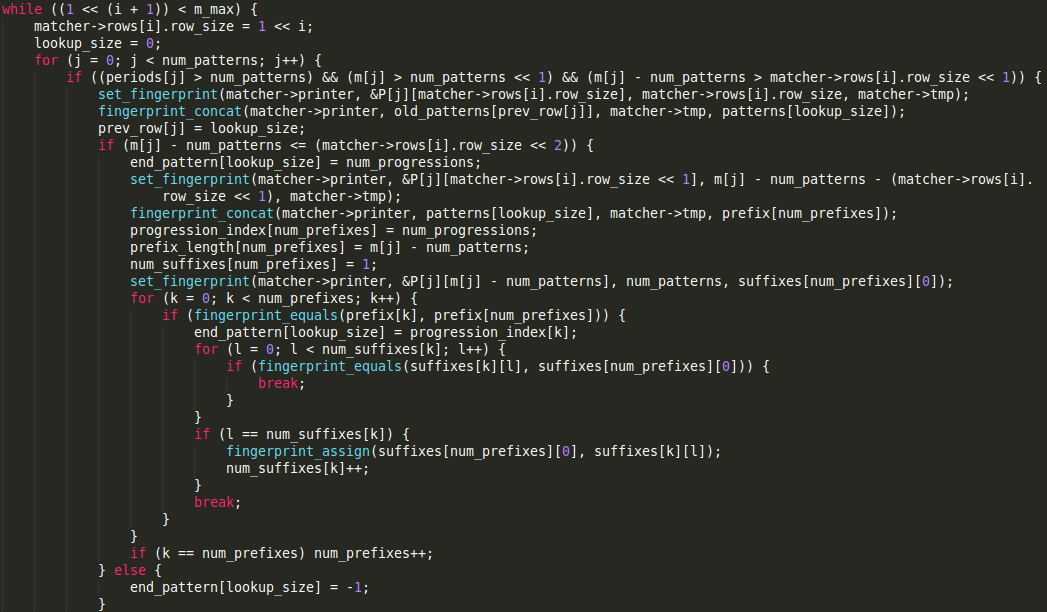
\includegraphics[scale=0.25]{complex_code}\footnote{\url{https://github.com/djmylt/dict_matching/blob/master/dict_matching.h}}
\end{frame}

\begin{frame}
\frametitle{Solution: Approximate!}
Let $f$ and $g$ be functions over the real numbers. We say that:

$$f(n) \in O(g(n)) \text{ iff } \exists c > 0, n_0 \geq 0 \text{ s.t. } \forall n \geq n_0, f(n) \leq c \cdot g(n)$$

$$f(n) \in \Omega(g(n)) \text{ iff } \exists c > 0, n_0 \geq 0 \text{ s.t. } \forall n \geq n_0, f(n) \geq c \cdot g(n)$$

$$f(n) \in \Theta(g(n)) \text{ iff } \exists c_1, c_2 > 0, n_0 \geq 0 \text{ s.t. } \forall n \geq n_0, c_1 \cdot g(n) \leq f(n) \leq c_2 \cdot g(n)$$
\end{frame}

\begin{frame}
\frametitle{Examples}
Prove each of the following statements:

$$n \in O(n^2)$$
$$2^n \in \Omega(n^2)$$
$$n \in \Theta(2n)$$
\end{frame}

\begin{frame}[noframenumbering]
\frametitle{Examples}
Prove each of the following statements:

$$n \in O(n^2): c = 1, n_0 = 0$$
$$2^n \in \Omega(n^2)$$
$$n \in \Theta(2n)$$
\end{frame}

\begin{frame}[noframenumbering]
\frametitle{Examples}
Prove each of the following statements:

$$n \in O(n^2): c = 1, n_0 = 0$$
$$2^n \in \Omega(n^2): c = 1, n_0 = 1$$
$$n \in \Theta(2n)$$
\end{frame}

\begin{frame}[noframenumbering]
\frametitle{Examples}
Prove each of the following statements:

$$n \in O(n^2): c = 1, n_0 = 0$$
$$2^n \in \Omega(n^2): c = 1, n_0 = 1$$
$$n \in \Theta(2n): c_1 = 0.5, c_2 = 1, n_0 = 0$$
\end{frame}

\begin{frame}
\frametitle{Time Complexity Classes}
Let $t: \mathbb{N} \to \mathbb{R}$ be a function.

$\mathrm{TIME}(t(n))$ is all the languages that can be decided by a $TM$ in $O(t(n))$ time.

$\mathrm{NTIME}(t(n))$ is all the languages that can be decided by a $NTM$ in $O(t(n))$ time.
\end{frame}

%------------------------------------------------
\section{Summary of part one}
%------------------------------------------------

\begin{frame}
\frametitle{Summary of part one}
\begin{itemize}
    \item What is a computer? {\em Deterministic Turing Machine, Nondeterministic Turing Machine}
    \item What is a problem? {\em Deciding if a word is in a language, verifying that a word is in a language}
    \item How do we measure difficulty? {\em Upper bound of time for an input of length $n$}
\end{itemize}
\end{frame}

%------------------------------------------------
\section{End of part one}
%------------------------------------------------

\begin{frame}
\frametitle{End of part one}
\begin{center}
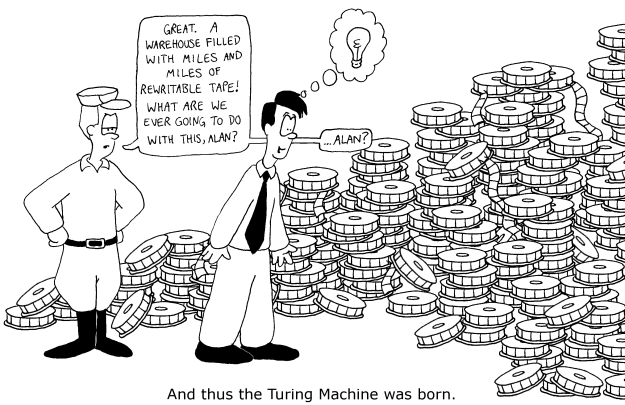
\includegraphics{turing_comic}\footnote{\url{http://www.cs.utah.edu/~draperg/cartoons/2005/turing.html}}
\end{center}
\end{frame}

%------------------------------------------------
\section{Structure of part two}
%------------------------------------------------

\begin{frame}
\frametitle{Structure of part two}
\begin{itemize}
    \item Putting it all together!
    \item ...only to get another (very difficult) problem.
    \item How might we try to solve this new problem?
\end{itemize}
\end{frame}

%------------------------------------------------
\section{Complexity classes}
%------------------------------------------------

\begin{frame}
\frametitle{Complexity Classes}
Now that we have provided our definitions for a computer, a problem and performance, we can look at what problems can be solved under these restrictions.

These are called {\em complexity classes}.
\end{frame}

\begin{frame}
\frametitle{Deterministic polynomial time}
One example of a complexity class is the set of languages that can be decided by a $TM$ in polynomial time.

$$\bigcup_{k = 0}^{\inf} \mathrm{TIME}(n^k)$$

We shall refer to the set of these problems as $P$.
\end{frame}

\begin{frame}
\frametitle{Nondeterministic polynomial time}
One example of a complexity class is the set of languages that can be decided by a $NTM$ in polynomial time.

$$\bigcup_{k = 0}^{\inf} \mathrm{NTIME}(n^k)$$

We shall refer to the set of these problems as $NP$.

We can also define $NP$ as the set of languages that can be verified by a $TM$ in polynomial time.
\end{frame}

\begin{frame}
\frametitle{From nondeterminism to verification}
Recall the computation tree for an $NTM$.

We label each branch with some integer.

Our certificate $c$ is now the polynomial length sequence of integers that lead to the accepting state.
\end{frame}

\begin{frame}
\frametitle{From verification to nondeterminism}
Since the verifier runs in polynomial time, the certificate must be polynomial in length.

We use nondeterminism to brute force the certificate.

And then run the verifier on every certificate.
\end{frame}

\begin{frame}
\frametitle{Structure of part two}
\begin{itemize}
    \item Putting it all together! {\em Complexity classes, $P, NP$}
    \item ...only to get another (very difficult) problem.
    \item How might we try to solve this new problem?
\end{itemize}
\end{frame}

%------------------------------------------------
\section{The $P$ versus $NP$ problem}
%------------------------------------------------

\begin{frame}
\frametitle{Exercise Left For the Student}
\centerline{Does $P=NP$?}
\end{frame}

\begin{frame}
\frametitle{The $P$ versus $NP$ problem}
Arguably first proposed by G\"{o}del in a letter to von Neumann in 1956.\footnote{\url{https://ecommons.cornell.edu/bitstream/handle/1813/6910/89-994.pdf}}

First stated formally by Cook in 1971.

Solving the problem will earn you a million dollars, courtesy of the Clay Mathematics Institute.\footnote{\url{http://www.claymath.org/millennium-problems/p-vs-np-problem}}
\end{frame}

\begin{frame}
\frametitle{The easy side: $P \subseteq NP$}

Recall that any $TM$ is by definition nondeterministic.

Likewise, any polynomial-time $TM$ is also nondeterministic.

Hence $P \subseteq NP$.
\end{frame}

\begin{frame}
\frametitle{The easy side: $P \subseteq NP$}

Alternative proof (using verification):

Let $TM\, M$ decide $L$ in polynomial time. Define $V$ as follows:

\begin{algorithm}[H]
$V(w, c):$\\
\If{$M(w)$ accepts}{
    {\bf accept}
}
\Else{
    {\bf reject}
}
\end{algorithm}

$V$ verifies $L$ in polynomial time. Hence $P \subseteq NP$.
\end{frame}

\begin{frame}
\frametitle{The harder side: Is $NP \subseteq P$}

Another way to think of this problem: {\em If a problem can be easily verified, can it be easily solved?}
\end{frame}

\begin{frame}
\frametitle{How might we answer this question?}

Why not look at the hardest problems in $NP$?

If $P = NP$, then even the hardest problems in $NP$ will be solvable in polynomial time.

And if $P \subset NP$, then these are the problems that won't have a polynomial time solution, as could be checked by lower-bound analysis.

But how can we determine the hardest problems in $NP$?
\end{frame}

\begin{frame}
\frametitle{Summary of part two}
\begin{itemize}
    \item Putting it all together! {\em Complexity classes, $P, NP$}
    \item ...only to get another (very difficult) problem. {\em Are easy to verify problems easy to solve?}
    \item How might we try to solve this new problem?
\end{itemize}
\end{frame}

%------------------------------------------------
\section{Completeness}
%------------------------------------------------

\begin{frame}
\frametitle{Polynomial time reducible}

Take two languages $A$ and $B$. We say that $A \leq_p B$ iff $\exists TM\, M$ such that:

\begin{itemize}
	\item $\forall w \in A, M(w) \in B$
	\item $\forall w \notin A, M(w) \notin B$
	\item and $M$ runs in worst-case $O(p(n))$ time for some polynomial $p$, where $n = |w|$
\end{itemize}

Note that this property is transitive: $A \leq_p B \text{ and } B \leq_q C \to A \leq_{p + q} C$

\end{frame}

\begin{frame}
\frametitle{$NP\text{-Complete}$}

A language $B$ is $NP\text{-Complete}$ iff:

\begin{itemize}
	\item $B \in NP$
	\item and $\forall A \in NP, A \leq_p B$
\end{itemize}

If one $NP\text{-Complete}$ language is proven to be in $P$, then every $NP$ problem is also in $P$.
\end{frame}

\begin{frame}
\frametitle{Problem: There are lots of $NP$ problems}
We know that any problem in $NP$ can be decided in polynomial time by an $NTM$.

So can we convert an $NTM$ to some other problem?
\end{frame}

\begin{frame}
\frametitle{Satisfiable boolean formulae}
Take a boolean formula $f = a \vee b \wedge \bar{c}$.

We say that $f$ is {\em satisfiable} if we can assign $0$ or $1$ to each variable such that $f = 1$.

Examples:
\begin{itemize}
	\item $f$ is satisfiable: $(a = 1, b = 1, c = 0)$
	\item but $f' = x \wedge \bar{x}$ is not satisfiable
\end{itemize}

We call $SAT$ the language of all satisfiable boolean formulae.
\end{frame}

\begin{frame}
\frametitle{$SAT \in NP$}
$SAT$ can be verified in polynomial time:

\begin{itemize}
	\item Make the certificate the values we assign to each variable.
	\item Have $V$ substitute the value for each variable into the formula.
	\item Accept if the formula evaluates to $1$, otherwise reject.
\end{itemize}
\end{frame}

\begin{frame}
\frametitle{Cook-Levin Theorem}
Cook showed that any $NTM\, M$ that halts in polynomial time can be converted to a polynomial length boolean formula such that:

\begin{itemize}
	\item If $M$ accepts, then the formula is satisfiable
	\item and if $M$ rejects, then the formula cannot be satisfied.
\end{itemize}

As a result, it was proven that $SAT \in NP\text{-Complete}$.
\end{frame}

\begin{frame}
\frametitle{Proving other $NP\text{-Complete}$ problems}

Now that we have one $NP\text{-Complete}$ problem, proving others is a lot easier.

Recall that polynomial-time reducibility is transitive.

So we can now provide a recursive definition. $B \in NP\text{-Complete}$ iff:

\begin{itemize}
	\item $B = SAT$
	\item or $B \in NP \text{ and } \exists A \in NP\text{-Complete s.t. } A \leq_p B$
\end{itemize}
\end{frame}

\begin{frame}
\frametitle{Other $NP\text{-Complete}$ problems}
\begin{itemize}
	\item<1-> $3SAT$
	\item<2-> Hamiltonian graphs
	\item<3-> Cliques
	\item<4-> Knapsack
	\item<5-> Tetris
	\item<6-> Lemmings
	\item<7-> Super Mario Bros
	\item<8-> Bejeweled
	\item<9-> Candy Crush Saga
	\item<10-> Flood-It
\end{itemize}
\end{frame}

%------------------------------------------------
\section{Summary of part two}
%------------------------------------------------

\begin{frame}
\frametitle{Summary of part two}
\begin{itemize}
    \item Putting it all together! {\em Complexity classes, $P, NP$}
    \item ...only to get another (very difficult) problem. {\em Are easy to verify problems easy to solve?}
    \item How might we try to solve this new problem? {\em $NP\text{-Complete}$ problems}
\end{itemize}
\end{frame}

%------------------------------------------------
\section{Beyond $P$ and $NP$}
%------------------------------------------------

\begin{frame}
\frametitle{What else is there?}
Recall our three questions from part one:
\begin{itemize}
    \item What is a computer?
    \item What is a problem?
    \item How do we measure difficulty?
\end{itemize}
What if we answered these differently?
\end{frame}

\begin{frame}
\frametitle{How do we measure difficulty?}
Exponential time: $EXP$

Linear time: $LIN$

Space complexity: $PSPACE, EXPSPACE$

Sublinear working space: $L$
\end{frame}

\begin{frame}
\frametitle{What is a problem?}
Computational problems: $NP\text{-Hard}$

Counting problems: $\#P$

Complementary problems: $\text{co-}NP$
\end{frame}

\begin{frame}
\frametitle{What is a computer?}
Probabilistic Turing Machines: $BPP, RP$

Postselection: $\text{Post-}BPP$

Parallel Computing: $NC$

Talking to another, more powerful computer: $MA, IP$

Oracles: $\Delta_iP, \Pi_iP, \Sigma_iP, PH$

Advice: $P/poly, P/log$

Quantum computers:  $EQP, BQP$

Time travel: $P_{CTC}$
\end{frame}

\begin{frame}
\frametitle{This is only the beginning}
There are many more complexity classes out there, and very quickly relating them in a simple equation like this:

$$P \subseteq NP$$

Becomes this:

$$L \subseteq NL \subseteq P \subseteq NP \subseteq PSPACE = NPSPACE = IP = P_{CTC} \subseteq EXP \subseteq EXPSPACE$$
\end{frame}

\begin{frame}
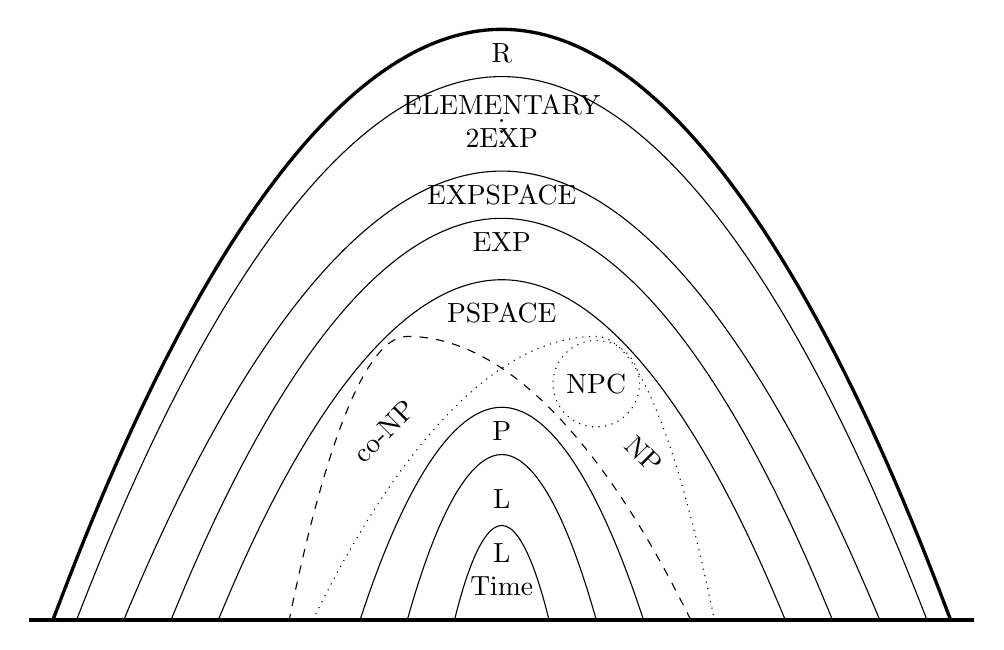
\begin{tikzpicture}
\pgftransformscale{.6}

%%% HELP LINES - uncomment to design/extend
% \draw[step=1cm,gray,very thin] (-10,0) grid (10,12);
% \node at (0,0) {\textbf{(0,0)}};

%% Horizontal bar
\draw[very thick] (10,0) -- (-10,0);

% LOG TIME
\draw (-1,0) parabola bend (0,2) (1,0) ;
\node at (0,1) {
	\begin{tabular}{c}
	L \\ Time
	\end{tabular}
};

% LOG SPACE
\draw (-2,0) parabola bend (0,3.5) (2,0);
\node at (0,2.5) {
	\begin{tabular}{c}
	L
	\end{tabular}
};

% PTIME
\draw (-3,0) parabola bend (0,4.5) (3,0);
\node at (0,4) {P};

% NP
\draw[dotted] (-4,0) parabola bend (2,6) (4.5,0);
\node[rotate=-45] at (3,3.5) {NP};

% NP-complete
\node[circle,dotted,draw] at (2,5) {NPC};

% Co-NP
\draw[dashed] (4,0) parabola bend (-2,6) (-4.5,0);
\node[rotate=45] at (-2.5,4) {co-NP};

% PSPACE
\draw (-6,0) parabola bend (0,7.2) (6,0);
\node at (0,6.5) {PSPACE};

% EXPTIME
\draw (-7,0) parabola bend (0,8.5) (7,0);
\node at (0,8) {EXP};

% EXPTIME
\draw (-8,0) parabola bend (0,9.5) (8,0);
\node at (0,9) {EXPSPACE};

% ELEMENTARY
\draw (-9,0) parabola bend (0,11.5) (9,0);
\node at (0,10.5) {$\vdots$};
\node[anchor=north] at (0,11.4) {
	\begin{tabular}{c}
		ELEMENTARY \\
		2EXP
	\end{tabular}
};

% RECURSIVE
\draw[very thick] (-9.5,0) parabola bend (0,12.5) (9.5,0);
\node at (0,12) {R};
\end{tikzpicture}\footnote{\url{http://www.texample.net/tikz/examples/complexity-classes/}}
\end{frame}

\begin{frame}
\frametitle{Open problems in complexity theory}
\begin{itemize}
	\item<1-> Does $P = NP$?
	\item<2-> Does $L = NL$?
	\item<3-> Does $BPP = P$?
	\item<4-> Does $BQP = BPP$?
	\item<5-> Does $NC = P$?
	\item<6-> Does $P = PSPACE$?
	\item<7-> Does $NP = \text{co-}NP$?
	\item<8-> And lots more...
\end{itemize}
\end{frame}

%------------------------------------------------
\section{The end}
%------------------------------------------------

\begin{frame}
\begin{center}
\frametitle{The end}
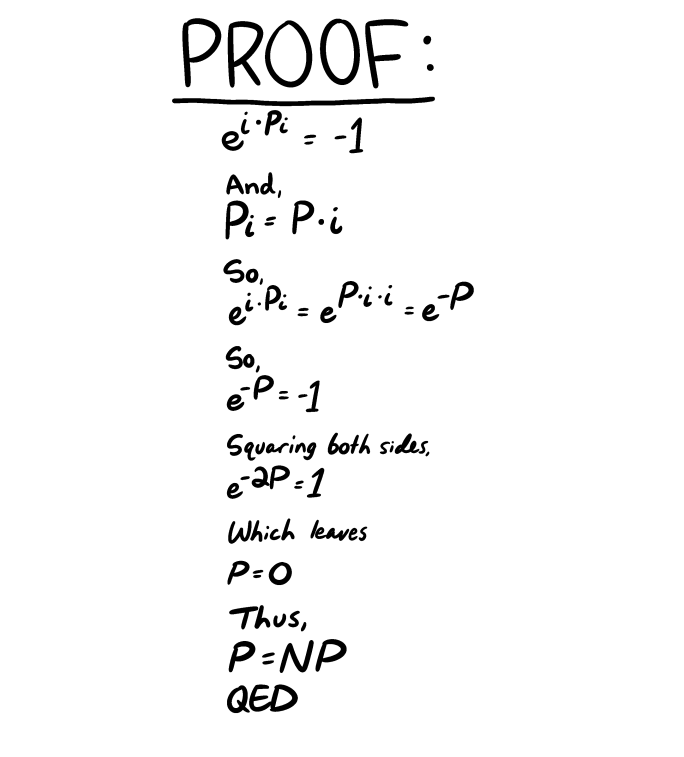
\includegraphics[scale=0.2]{smbc_comic}\footnote{\url{http://www.smbc-comics.com/?id=3919}}
\end{center}
\end{frame}

\begin{frame}
\begin{center}
\frametitle{The end}
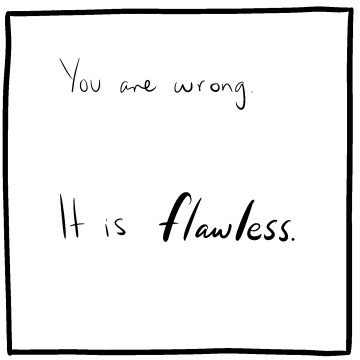
\includegraphics[scale=0.5]{smbc_comic_votey}\footnote{\url{http://www.smbc-comics.com/?id=3919}}
\end{center}
\end{frame}

\begin{frame}
\frametitle{Suggested books}
\begin{itemize}
	\item {\em Quantum Computing Since Democritus} by Scott Aaronson offers a broad overview of many complexity classes
	\item {\em Introduction to the Theory of Computation} by Michael Sipser is the recommended textbook for most computability and complexity theory courses
\end{itemize}
\end{frame}

\begin{frame}
\frametitle{Suggested papers}
\begin{itemize}
	\item {\em On Computable Numbers, with an Application to the Entscheidungsproblem} by Alan Turing is Turing's PhD thesis, which provides the original definition of Turing Machines, a formal definition of the Universal Turing Machine, and a proof that the Halting problem is undecidable
	\item {\em The Complexity of Theorem Proving Procedures} by Stephen Cook provides the proof that $SAT \in NP\text{-Complete}$
	\item {\em Reducibility Among Combinatorial Problems} by Richard Karp provides 21 of the earliest problems proven to be $NP\text{-Complete}$
\end{itemize}
\end{frame}

\begin{frame}
\frametitle{Suggested websites}
\begin{itemize}
	\item \url{https://complexityzoo.uwaterloo.ca/} is a Wiki originally developed by Scott Aaronson, which provides a list of every complexity class ever stated
\end{itemize}
\end{frame}

%----------------------------------------------------------------------------------------

\end{document} 
